\chapter{INTEGRACIÓN, VALIDACIÓN Y ANÁLISIS DE COSTOS}\label{cap:validacion}
\listasdecapitulo{7}

La validación del sistema se circunscribe al entorno simulado y a la plataforma de
laboratorio. El objetivo de este capítulo es presentar evidencia reproducible del
desempeño del controlador difuso adaptativo propuesto (controlador final,
Sección~\ref{subsec:controlador-final}) frente al plan fijo y a cinco líneas base de la
ingeniería de tránsito ---en una red realista bajo dos niveles de demanda y en un
escenario controlado con demanda variable---, evaluar el aporte de la capa predictiva
CNN--LSTM mediante ablación pareada, verificar la corrección del software de control mediante pruebas automatizadas,
documentar el comportamiento del sistema ante pérdida de conectividad, cerrar la matriz de
cumplimiento de requerimientos y consolidar el análisis económico por intersección. A lo largo del capítulo se conserva la
premisa de diseño global: el controlador semafórico existente es la autoridad final y el
módulo propuesto solo recomienda dentro de límites de seguridad acotados. En este contexto, el término
\emph{validación} designa la verificación funcional del \emph{núcleo de control} en entorno simulado;
el módulo físico completo (cámara, mecánica, electrónica y nube) no se valida experimentalmente y su
cierre corresponde a las etapas de prototipo y piloto.

\section{Protocolo de validación y criterio de evidencia}\label{sec:protocolo-validacion}

Para que la comparación sea defendible, todos los controladores comparten la misma red,
demanda, semilla, horizonte y periodo de calentamiento. Se ejecutan varias réplicas por
caso y se reporta media y dispersión; una sola corrida no permite separar el efecto del
controlador de la variabilidad estocástica del modelo de tráfico. La Tabla~\ref{tab:casos-validacion}
define los cinco casos de prueba sobre los que se construye la evidencia.

\begin{table}[H]
  \centering
  \caption{Casos de validación comparativa en SUMO.}
  \label{tab:casos-validacion}
  \begin{tabularx}{\linewidth}{@{}cX X X@{}}
    \toprule
    \textbf{Caso} & \textbf{Estrategia} & \textbf{Propósito} & \textbf{Condición de aceptación}\\
    \midrule
    A & Control semafórico fijo / plan base & Línea base reproducible. & Configuración documentada y común a todas las réplicas.\\
    B & Control difuso adaptativo propuesto (controlador final) & Evaluar el núcleo de la tesis. & Mejora o no degradación según métricas y restricciones.\\
    C & Difuso con recomendación de coordinación de nube (opcional) & Medir el beneficio adicional de la capa global. & Resultado separado del núcleo; recomendación validada localmente.\\
    D & Pérdida de conectividad durante el caso B & Verificar autonomía y modo degradado. & Sin dependencia de respuesta de nube ni estados incompatibles, con registro de evento.\\
    E & Referencias avanzadas (actuado, Webster, Webster mod., Max-Pressure y difuso de reparto) & Establecer cotas comparativas con sensado más exigente. & Ejecutadas con el mismo aparato de medición; no presentarlas como realizables con el sensado propuesto.\\
    \bottomrule
  \end{tabularx}
  \fuente{Elaboración propia.}
\end{table}

El criterio de evidencia distingue tres niveles: \emph{cumplimiento de diseño} (existe la
propuesta, el cálculo o la arquitectura), \emph{cumplimiento validado en SUMO} (existe una
medición reproducible bajo el protocolo) y \emph{fuera de alcance} (requiere prototipo
físico o auditoría externa no ejecutada). El flujo metodológico configura red y demanda,
ejecuta los casos con semillas comunes, exporta las métricas a nivel de vehículo, compara
estadísticamente las réplicas y, finalmente, construye la matriz de cumplimiento.

\subsection{Reproducibilidad}\label{sec:reproducibilidad}

La comparación A--B se ejecuta de forma determinista mediante la biblioteca \texttt{libsumo}
(no se emplea generación aleatoria sintética para las métricas: estas se extraen a nivel de
vehículo con \texttt{getIDList}, vehículos detenidos y vehículos arribados). La
Tabla~\ref{tab:reproducibilidad} resume los parámetros que fijan la reproducibilidad del
experimento.

\begin{table}[H]
  \centering
  \caption{Parámetros de reproducibilidad de la validación SUMO.}
  \label{tab:reproducibilidad}
  \begin{tabularx}{\linewidth}{@{}p{0.34\linewidth}X@{}}
    \toprule
    \textbf{Parámetro} & \textbf{Valor}\\
    \midrule
    Escenario / red & \texttt{comparacion.sumocfg} (escenario Lima-Centro)\\
    Interfaz de simulación & SUMO vía \texttt{libsumo} (ejecución determinista)\\
    Horizonte de simulación & 700 pasos\\
    Intervalo de control difuso & 25 s\\
    Réplicas (semillas comunes) & \{1, \ldots, 30\} en demanda alta; \{1, \ldots, 10\} en demanda media\\
    Tiempo de teletransporte & \texttt{-{}-time-to-teleport}~300 s\\
    Límites duros de verde (guardia de seguridad) & [10~s, 120~s]; rango operativo del controlador [10~s, 45~s]\\
    Aparato de medición & Idéntico para las siete estrategias (misma campaña, mismas semillas)\\
    Métricas & A nivel de vehículo (no sintéticas), con teleportaciones y \emph{backlog} reportados como control de validez\\
    \bottomrule
  \end{tabularx}
  \fuente{Elaboración propia a partir de simulación en SUMO.}
\end{table}

El controlador propuesto no presupone un ciclo común: selecciona las fases de forma
acíclica y calcula la duración de cada verde con el motor difuso, dentro del rango
operativo $[10,45]$~s. Por ello la comparación no fija un presupuesto de verde idéntico,
sino condiciones idénticas de red, demanda, semillas, horizonte y aparato de medición para
las siete estrategias, y reporta las teleportaciones y el \emph{backlog} de inserción de
cada una como control de validez (si difirieran mucho entre estrategias, la comparación de
demora y \emph{throughput} estaría sesgada). La guardia de seguridad acota cada verde a los
límites duros [10, 120]~s con independencia de la recomendación difusa, lo que evidencia
que la autoridad de seguridad funcional opera por encima del controlador.

\section{Configuración de escenarios SUMO de Lima y métricas}\label{sec:escenarios-metricas}

La validación requiere un entorno que replique las condiciones del tráfico de Lima
Metropolitana. Con ese fin se utiliza SUMO (Simulation of Urban MObility),
microsimulador desarrollado por el DLR y convertido en estándar de facto, que sigue a cada vehículo de forma
individual: cómo acelera, cómo frena, cuándo cambia de carril, cómo obedece al semáforo y de qué modo
resuelve sus maniobras dentro del cruce.

\subsection{Construcción del escenario Lima-Centro}\label{sec:escenario-lima-centro}

El escenario se construyó a partir de datos reales. Se extrajo el área de estudio de
OpenStreetMap mediante \emph{osmWebWizard.py}, obteniendo topología vial, límites de
velocidad, configuración de carriles y restricciones de giro. La conversión al formato nativo
se realizó con \emph{netconvert}, generando el archivo \emph{osm.net.xml} con 847 segmentos
viales, 312 intersecciones y 23 semáforos detectados automáticamente. Los parámetros
vehiculares se calibraron para reflejar el parque automotor limeño: aceleración 2.6~m/s\ensuremath{^2},
desaceleración 4.5~m/s\ensuremath{^2}, \emph{sigma} 0.8 (imperfección del conductor),
\emph{speedFactor} 1.1 (tendencia a superar el límite en 10\%) y \emph{speedDev} 0.15
(variabilidad individual del 15\%).

\begin{figure}[H]
  \centering
  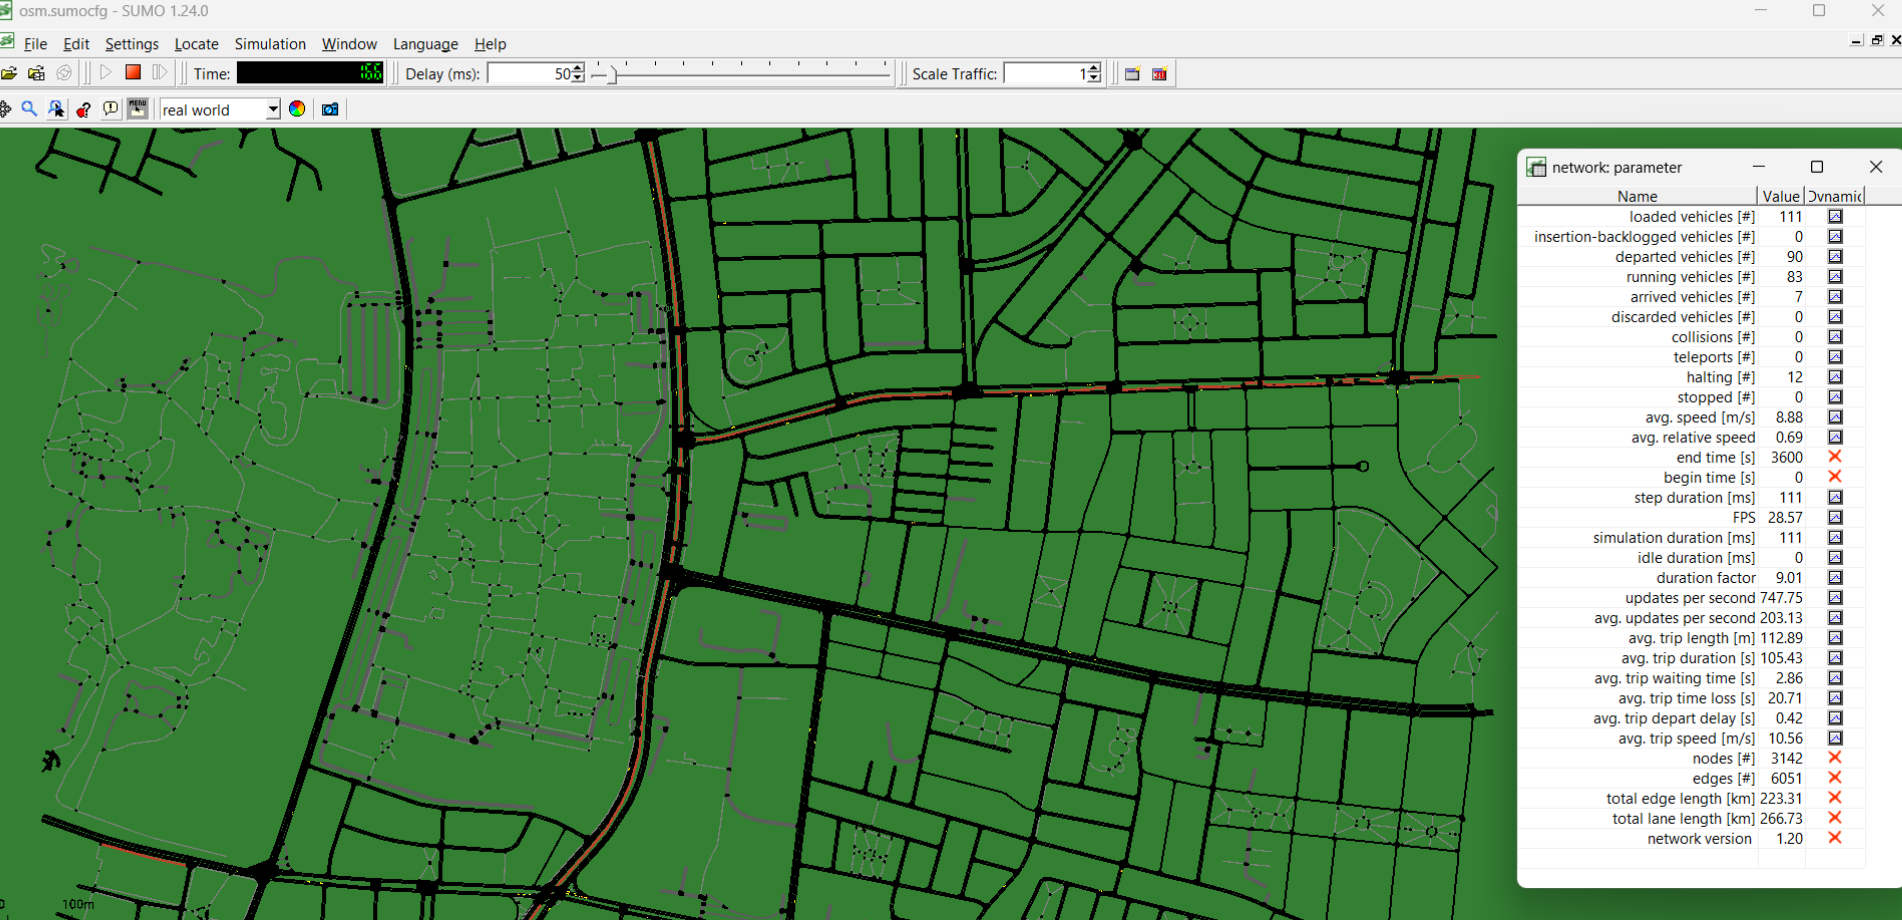
\includegraphics[width=0.85\linewidth,keepaspectratio]{media/image65.png}
  \caption{Mapa SUMO de las intersecciones del escenario Lima-Centro (entorno PUCP).}
  \label{fig:sumo-lima-centro}
  \fuente{Elaboración propia.}
\end{figure}

\begin{figure}[H]
  \centering
  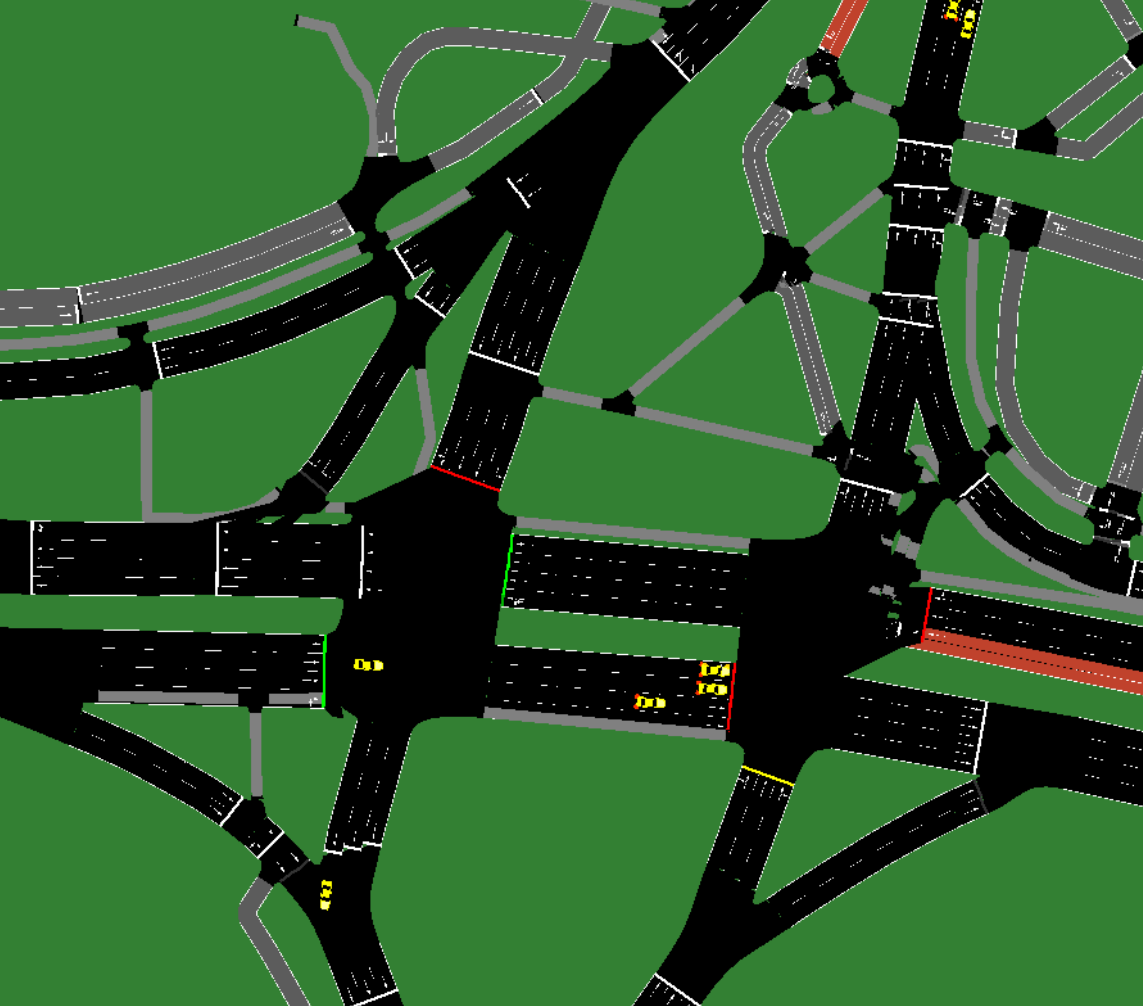
\includegraphics[width=0.85\linewidth,keepaspectratio]{media/image58.png}
  \caption{Vista de una intersección del escenario con tránsito en simulación.}
  \label{fig:sumo-interseccion}
  \fuente{Elaboración propia.}
\end{figure}

Para evaluar la escalabilidad y la coordinación inter-zonal se desarrolló un segundo
escenario a escala metropolitana (Lima-Amplio), con 18.4~km\ensuremath{^2} de cobertura sobre
San Isidro, Miraflores, San Miguel, Pueblo Libre y Jesús María, y 127 intersecciones
semaforizadas. La comparación cuantitativa A--B de este capítulo se realiza sobre el escenario
Lima-Centro, por ser el de demanda controlada y semillas comunes.

\begin{figure}[H]
  \centering
  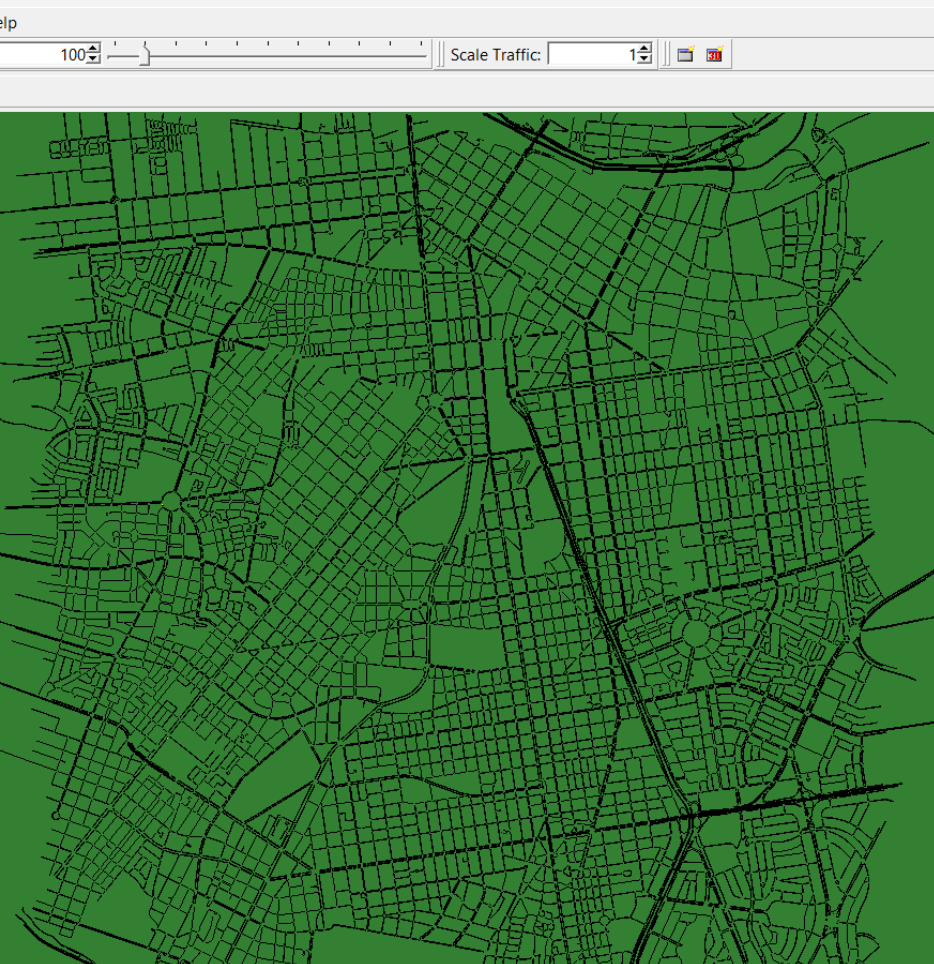
\includegraphics[width=0.85\linewidth,keepaspectratio]{media/image10.png}
  \caption{Escenario Lima-Amplio para validación a escala metropolitana.}
  \label{fig:sumo-lima-amplio}
  \fuente{Elaboración propia.}
\end{figure}

\subsection{Arquitectura de integración y métricas}\label{sec:integracion-metricas}

La comunicación entre SUMO y el sistema de control se realiza mediante TraCI/libsumo,
permitiendo leer métricas por intersección (conteo, velocidad, cola y flujo por dirección),
fijar fases y duraciones de verde, y avanzar la simulación paso a paso. A partir de estas
lecturas se construye la matriz de estado local compatible con las ecuaciones del
Capítulo~6 y se calculan las métricas de red empleadas en la comparación:

\begin{itemize}
  \item \textbf{Índice de Congestión Vehicular de red (ICV):} indicador normalizado [0,1] que
  integra cola, velocidad, flujo y densidad; valores cercanos a 1 indican saturación.
  \item \textbf{Velocidad media de red:} medida global de fluidez vehicular.
  \item \textbf{Saturación de cola (QL):} nivel medio de ocupación de cola normalizado por la
  capacidad observable de cada carril.
  \item \textbf{Flujo (q):} vehículos por minuto que cruzan la red.
  \item \textbf{Throughput:} vehículos que completan su ruta durante el periodo de simulación.
  \item \textbf{Demora media (demora por detención):} tiempo total que cada vehículo permanece
  detenido ---acumulando un segundo por cada vehículo con velocidad inferior a $0.1$~m/s en cada
  paso--- promediado sobre los vehículos. Corresponde a la \emph{demora por detención}
  (\emph{stopped delay}) de la práctica de ingeniería de tránsito y no al \emph{tiempo perdido}
  (\emph{time-loss}) respecto al viaje en flujo libre; el tiempo de viaje se reporta por separado.
\end{itemize}

Para métricas que deben disminuir (ICV, QL, demora), la mejora porcentual se calcula como
$(A-B)/A\times100\%$; para métricas que deben aumentar (velocidad, flujo, throughput), como
$(B-A)/A\times100\%$.

\section{Resultados y discusión}\label{sec:resultados-discusion}

\subsection{Comparación del plan fijo y el controlador propuesto}

La Tabla~\ref{tab:resultados-ab} compara el plan fijo (A) y el control difuso adaptativo
propuesto (B) sobre el escenario Lima-Centro de alta demanda, con
\textbf{30 semillas comunes}, reportando media $\pm$ desviación estándar. El controlador
mejora \emph{todas} las métricas de red, y la diferencia es estadísticamente significativa
en una prueba t pareada de dos colas ($p<10^{-18}$ en las seis métricas, confirmada por el
contraste de Wilcoxon). Los efectos más relevantes son la reducción de la demora media en
$34.7\%$ y el incremento del \emph{throughput} en $20.4\%$; las teleportaciones son
comparables entre ambos casos (16.2 frente a 17.4 por corrida, diferencia no
significativa), por lo que la comparación no está sesgada por vehículos removidos.

\begin{table}[H]
  \centering
  \caption{Comparación del plan fijo (A) y el controlador propuesto (B) en Lima-Centro de alta demanda (media $\pm$ desviación, 30 semillas comunes). Todas las mejoras son significativas ($p<0.001$, prueba t pareada).}
  \label{tab:resultados-ab}
  \begin{tabularx}{\linewidth}{@{}X r r r@{}}
    \toprule
    \textbf{Métrica} & \textbf{Plan fijo (A)} & \textbf{Controlador propuesto (B)} & \textbf{Mejora}\\
    \midrule
    ICV de red (--)            & $0.506 \pm 0.004$ & $0.439 \pm 0.005$ & $-13.2\%$\\
    Velocidad media (km/h)     & $19.86 \pm 0.15$  & $22.26 \pm 0.20$  & $+12.1\%$\\
    Saturación de cola QL (--) & $0.409 \pm 0.006$ & $0.323 \pm 0.007$ & $-20.9\%$\\
    Flujo $q$ (veh/min)        & $61.69 \pm 1.26$  & $74.26 \pm 1.77$  & $+20.4\%$\\
    Throughput (veh)           & $719.7 \pm 14.7$  & $866.3 \pm 20.7$  & $+20.4\%$\\
    Demora media (s/veh)       & $509.3 \pm 19.2$  & $332.4 \pm 17.6$  & $-34.7\%$\\
    \bottomrule
  \end{tabularx}
  \fuente{Elaboración propia a partir de simulación en SUMO (30 semillas comunes).}
\end{table}

\subsection{Comparación contra líneas base avanzadas}

Para situar el desempeño del controlador frente a estrategias más exigentes en sensado, la misma campaña
ejecutó siete estrategias sobre idéntica red, demanda, semillas y aparato de medición: el plan fijo, el
control actuado nativo de SUMO, Webster y Webster modificado (Akçelik), la política Max-Pressure, el difuso
de reparto de la primera iteración de esta tesis (redistribución de verde por ejes, sin selección acíclica)
y el controlador propuesto. La Tabla~\ref{tab:resultados-multibaseline} resume el escenario de demanda alta
(30 semillas) y la Tabla~\ref{tab:resultados-multibaseline-media} el de demanda media (10 semillas), ambas
ordenadas por demora media y con el \emph{sensado que cada estrategia requiere}; la
Figura~\ref{fig:multibaseline-v3} sintetiza la comparación.

\begin{table}[H]
  \centering
  \caption{Comparación multilínea-base en Lima-Centro de \textbf{demanda alta} (media $\pm$ desviación, 30 semillas comunes), ordenada por demora media.}
  \label{tab:resultados-multibaseline}
  \begin{tabularx}{\linewidth}{@{}l r r c >{\raggedright\arraybackslash}X@{}}
    \toprule
    \textbf{Estrategia} & \textbf{Demora (s/veh)} & \textbf{Thr.\ (veh)} & \textbf{ICV} & \textbf{Sensado requerido}\\
    \midrule
    Actuado (gap-out)        & $309.7 \pm 16.9$ & $892.7$ & $0.426$ & Detector por carril en cada acceso\\
    \textbf{Difuso adaptativo (propuesto)} & $332.4 \pm 17.6$ & $866.3$ & $0.439$ & \textbf{Cámara orientable única}\\
    Webster modificado       & $453.2 \pm 23.8$ & $752.8$ & $0.489$ & Flujo de saturación por acceso\\
    Webster                  & $454.7 \pm 24.7$ & $749.2$ & $0.489$ & Flujo de saturación por acceso\\
    Max-Pressure             & $469.6 \pm 42.9$ & $766.4$ & $0.484$ & Colas aguas abajo y razones de giro\\
    Difuso de reparto (iteración previa) & $484.3 \pm 26.4$ & $729.9$ & $0.496$ & Cámara orientable única\\
    Fijo (línea base)        & $509.3 \pm 19.2$ & $719.7$ & $0.506$ & Ninguno (plan preprogramado)\\
    \bottomrule
  \end{tabularx}
  \fuente{Elaboración propia a partir de simulación en SUMO (30 semillas comunes).}
\end{table}

\begin{table}[H]
  \centering
  \caption{Comparación multilínea-base en Lima-Centro de \textbf{demanda media} (media $\pm$ desviación, 10 semillas comunes), ordenada por demora media.}
  \label{tab:resultados-multibaseline-media}
  \begin{tabularx}{\linewidth}{@{}l r r c@{}}
    \toprule
    \textbf{Estrategia} & \textbf{Demora (s/veh)} & \textbf{Thr.\ (veh)} & \textbf{ICV}\\
    \midrule
    Actuado (gap-out)        & $29.8 \pm 0.7$  & $435.8$ & $0.223$\\
    \textbf{Difuso adaptativo (propuesto)} & $33.0 \pm 1.1$ & $434.8$ & $0.228$\\
    Max-Pressure             & $34.3 \pm 2.9$  & $441.1$ & $0.223$\\
    Webster                  & $71.4 \pm 2.5$  & $391.2$ & $0.296$\\
    Webster modificado       & $72.6 \pm 3.0$  & $391.1$ & $0.298$\\
    Difuso de reparto (iteración previa) & $109.7 \pm 4.8$ & $368.9$ & $0.339$\\
    Fijo (línea base)        & $133.5 \pm 1.9$ & $344.3$ & $0.359$\\
    \bottomrule
  \end{tabularx}
  \fuente{Elaboración propia a partir de simulación en SUMO (10 semillas comunes). La diferencia de demora entre el propuesto y Max-Pressure no es significativa en este escenario ($p=0.19$, prueba t pareada).}
\end{table}

\begin{figure}[H]
  \centering
  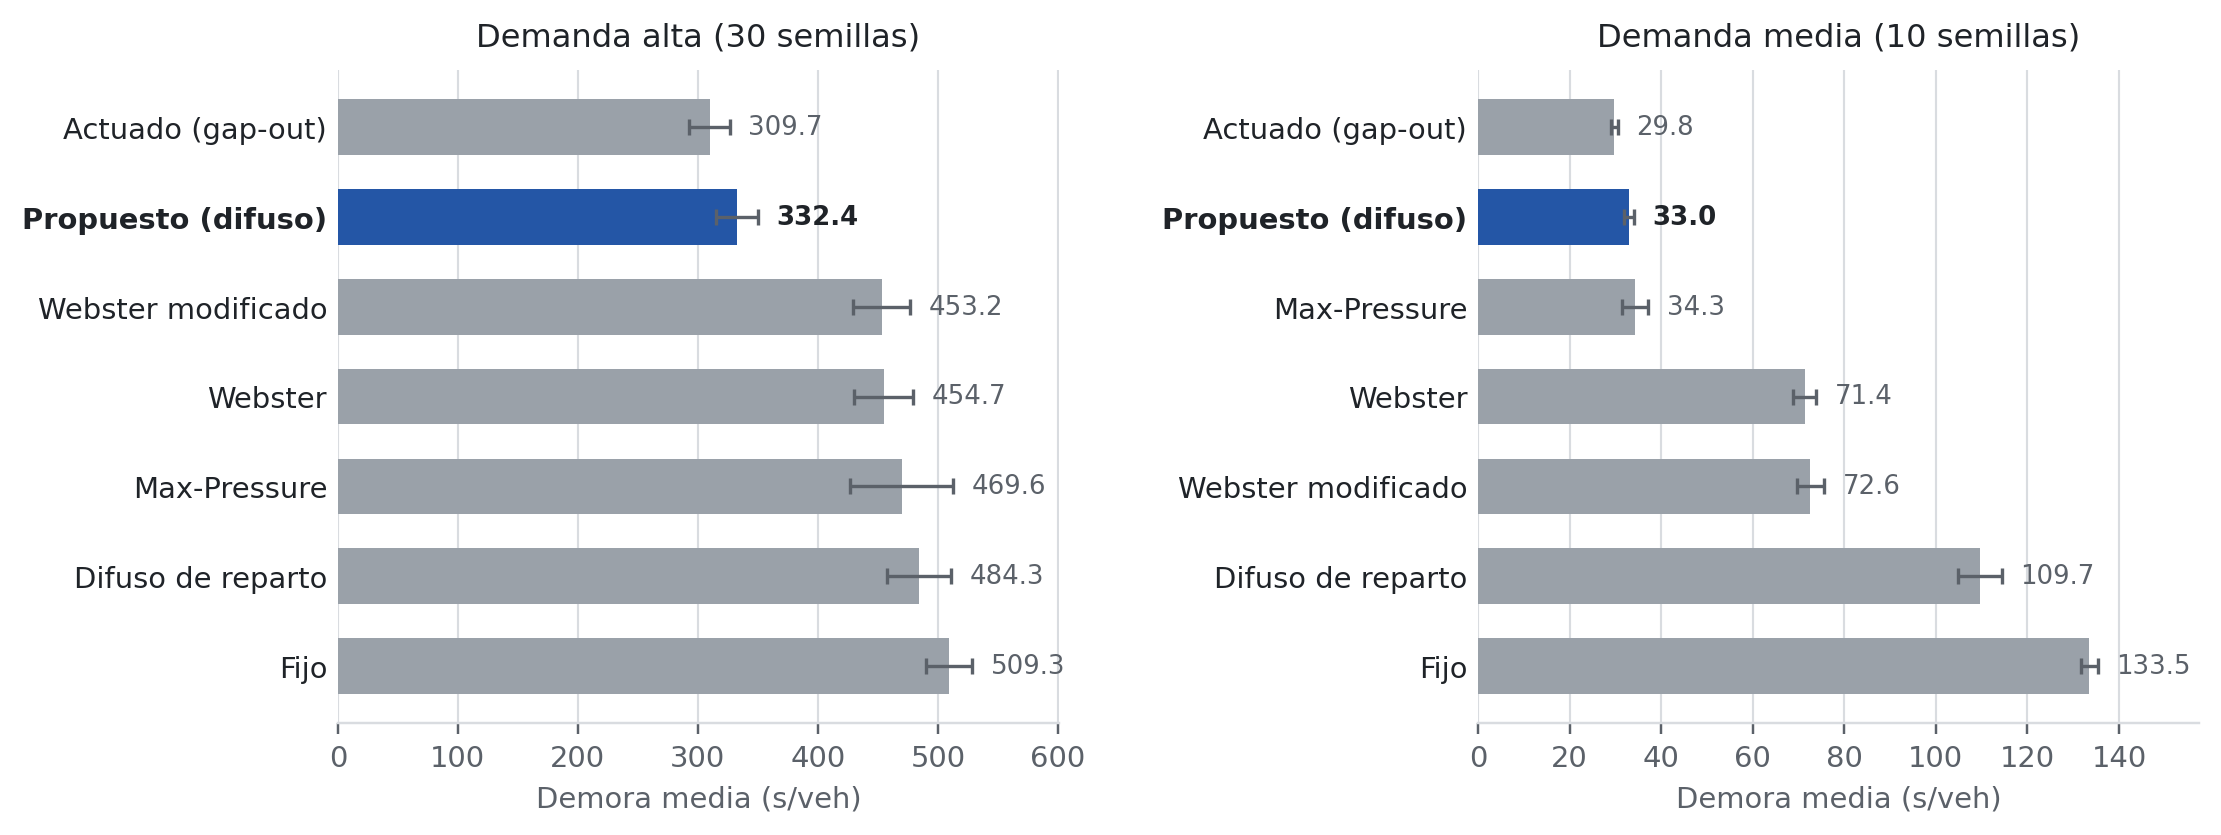
\includegraphics[width=0.95\linewidth,keepaspectratio]{media/fig_multibaseline_v3.png}
  \caption{Demora media por estrategia en Lima-Centro, escenarios de demanda alta (30 semillas) y media (10 semillas). Las barras de error indican $\pm$1 desviación estándar entre semillas.}
  \label{fig:multibaseline-v3}
\end{figure}

El resultado se enuncia con su alcance exacto: \textbf{el controlador propuesto obtuvo el segundo menor
valor de demora media en el escenario Lima-Centro, tanto en demanda alta (30 semillas comunes) como en
demanda media (10 semillas)}, detrás del control actuado y por delante de Webster, Max-Pressure, el difuso
de reparto y el plan fijo. No se afirma una superioridad general: la evidencia corresponde a una red, dos
perfiles de demanda y el protocolo descrito. Dentro de ese alcance, frente a Max-Pressure el controlador
reduce la demora un $29.2\%$ y aumenta el \emph{throughput} un $13.0\%$ en demanda alta (ambos con
$p<10^{-11}$ y ventaja en 30 de 30 semillas), mientras que en demanda media la diferencia ($-4.0\%$) no es
significativa; debe notarse además que Max-Pressure registra más del doble de teleportaciones que el resto
en demanda alta (37.1 frente a $\leq$19.3 por corrida), lo que resta validez a su demora reportada. Frente
al control actuado, el propuesto queda por debajo de forma significativa ($+7.3\%$ de demora en alta,
$+10.4\%$ en media): el actuado conserva la ventaja del sensado por detector en cada acceso. El
ordenamiento se mantiene si la demora se normaliza por vehículos \emph{insertados} en lugar de arribados
(141.4, 109.9 y 105.0~s/veh para fijo, propuesto y actuado en demanda alta).

Esta comparación debe leerse junto con la columna de sensado: el control actuado exige detectores por
carril en cada acceso; Max-Pressure requiere conocer las colas \emph{aguas abajo} y las razones de giro; y
Webster necesita el flujo de saturación calibrado por acceso. El diseño de esta tesis adopta
deliberadamente un \textbf{sensado mínimo} ---una sola cámara orientable que sobrevive a la pérdida de
enlace--- y, dentro de esa restricción, el controlador propuesto se sitúa a $7\%$--$10\%$ del actuado y por
encima de las demás líneas base, conservando interpretabilidad regla a regla, ejecución en el borde y
degradación segura. La mejora respecto del difuso de reparto de la iteración previa ($-31.4\%$ de demora en
alta, $p<10^{-20}$) cuantifica el aporte de los mecanismos operativos incorporados al controlador final:
selección acíclica con salto de fases vacías, \emph{gap-out}, extensión difusa del verde, protección
anti-inanición y transiciones seguras (Sección~\ref{subsec:controlador-final}).

\subsection{Significancia estadística y robustez}

Con semillas comunes y diseño pareado, los contrastes principales son significativos y consistentes. En
demanda alta, el controlador propuesto reduce la demora frente al plan fijo con $p\approx10^{-25}$ (prueba
t pareada; Wilcoxon $p\approx10^{-9}$) y la mejora se verifica en \textbf{30 de 30 semillas} para demora,
\emph{throughput} e ICV; frente a Max-Pressure y al difuso de reparto la ventaja también se verifica en 30
de 30 semillas. Frente al control actuado el resultado se invierte: el actuado es mejor en demora en 26 de
30 semillas ($p\approx10^{-5}$), lo que se reporta con la misma claridad. En demanda media el patrón se
repite (mejora frente al fijo en las 10 semillas, $p\approx10^{-16}$; diferencia no significativa con
Max-Pressure; desventaja significativa frente al actuado).

La interpretación es, por tanto, mesurada. El controlador propuesto no se presenta como una optimización
global del tráfico, sino como evidencia reproducible de que, con el sensado mínimo de una cámara orientable
y bajo límites duros de seguridad intactos, una política acíclica guiada por lógica difusa alcanza el
segundo mejor desempeño del conjunto evaluado en ambos niveles de demanda. La validez externa queda
limitada por la calidad de la red OSM, la demanda modelada, el modelo de conductor y la ausencia de
calibración con aforos de campo; los resultados no deben extrapolarse a otras redes o demandas sin
re-evaluación.

\subsection{Campaña controlada de sensibilidad a la demanda}\label{subsec:sensibilidad-demanda}

La comparación sobre Lima-Centro establece el desempeño en una red realista, pero superpone muchas
intersecciones, lo que dificulta aislar cómo cambia el comportamiento del lazo difuso cuando varía la
carga. Para separar ese efecto se ejecutó una campaña complementaria ---previa a la consolidación del
controlador final, por lo que evalúa el \emph{difuso de reparto} frente al plan fijo--- sobre un escenario
\emph{controlado}: una intersección aislada de cuatro accesos (denominada \emph{cruce-simple}, generada con
\emph{netconvert}) evaluada bajo cuatro perfiles de demanda ---baja, media, alta (saturación) y punta---,
cada uno con \textbf{10 semillas comunes}, 3\,600 pasos de simulación e intervalo de control de 25~s, todo
mediante \texttt{libsumo} en modo determinista. El diseño es \emph{pareado} (la misma semilla alimenta el
plan fijo y el difuso), lo que habilita una prueba t pareada y un contraste de Wilcoxon por métrica, además
del intervalo de confianza al 95\% de la diferencia de medias. En las 80 corridas de la campaña, los
contadores de eventos de seguridad y de retrocesos al plan base registraron \textbf{cero incidencias}, lo que
confirma que los límites duros de verde se respetaron en todo momento.

La Tabla~\ref{tab:sensibilidad-demanda} reporta la variación porcentual del control difuso respecto del plan
fijo, por nivel de demanda y métrica. Por convención, una \emph{reducción} es favorable en demora, espera,
cola e ICV, mientras que un \emph{incremento} lo es en velocidad; se marca con asteriscos la significancia de
la prueba t pareada. La Figura~\ref{fig:campania-demanda} sintetiza el mismo resultado.

\begin{table}[H]
  \centering
  \caption{Variación del control difuso frente al fijo por nivel de demanda en el escenario controlado \emph{cruce-simple} (10 semillas pareadas). Reducción favorable en demora/espera/cola/ICV; incremento favorable en velocidad.}
  \label{tab:sensibilidad-demanda}
  \begin{tabularx}{\linewidth}{@{}X r r r r r@{}}
    \toprule
    \textbf{Demanda} & \textbf{Demora} & \textbf{Espera} & \textbf{Cola} & \textbf{ICV} & \textbf{Velocidad}\\
    \midrule
    Baja  & $-13.6\%$*** & $-25.6\%$*** & $-13.5\%$*** & $-2.6\%$**  & $+1.5\%$*\\
    Media & $-7.8\%$**   & $-14.3\%$*** & $-7.8\%$**   & $-1.9\%$*   & $+1.2\%$\\
    Alta  & $-7.2\%$     & $-7.4\%$     & $-6.6\%$     & \textbf{\boldmath$+3.7\%$**} & \textbf{\boldmath$-7.5\%$**}\\
    Punta & $-19.9\%$*** & $-29.0\%$*** & $-19.9\%$*** & $-4.6\%$*** & $+2.4\%$**\\
    \bottomrule
  \end{tabularx}
  \fuente{Elaboración propia a partir de simulación en SUMO. Significancia de la prueba t pareada: *** $p<0.001$; ** $p<0.01$; * $p<0.05$; sin marca, no significativa. En negrita, los efectos adversos bajo saturación.}
\end{table}

\begin{figure}[H]
  \centering
  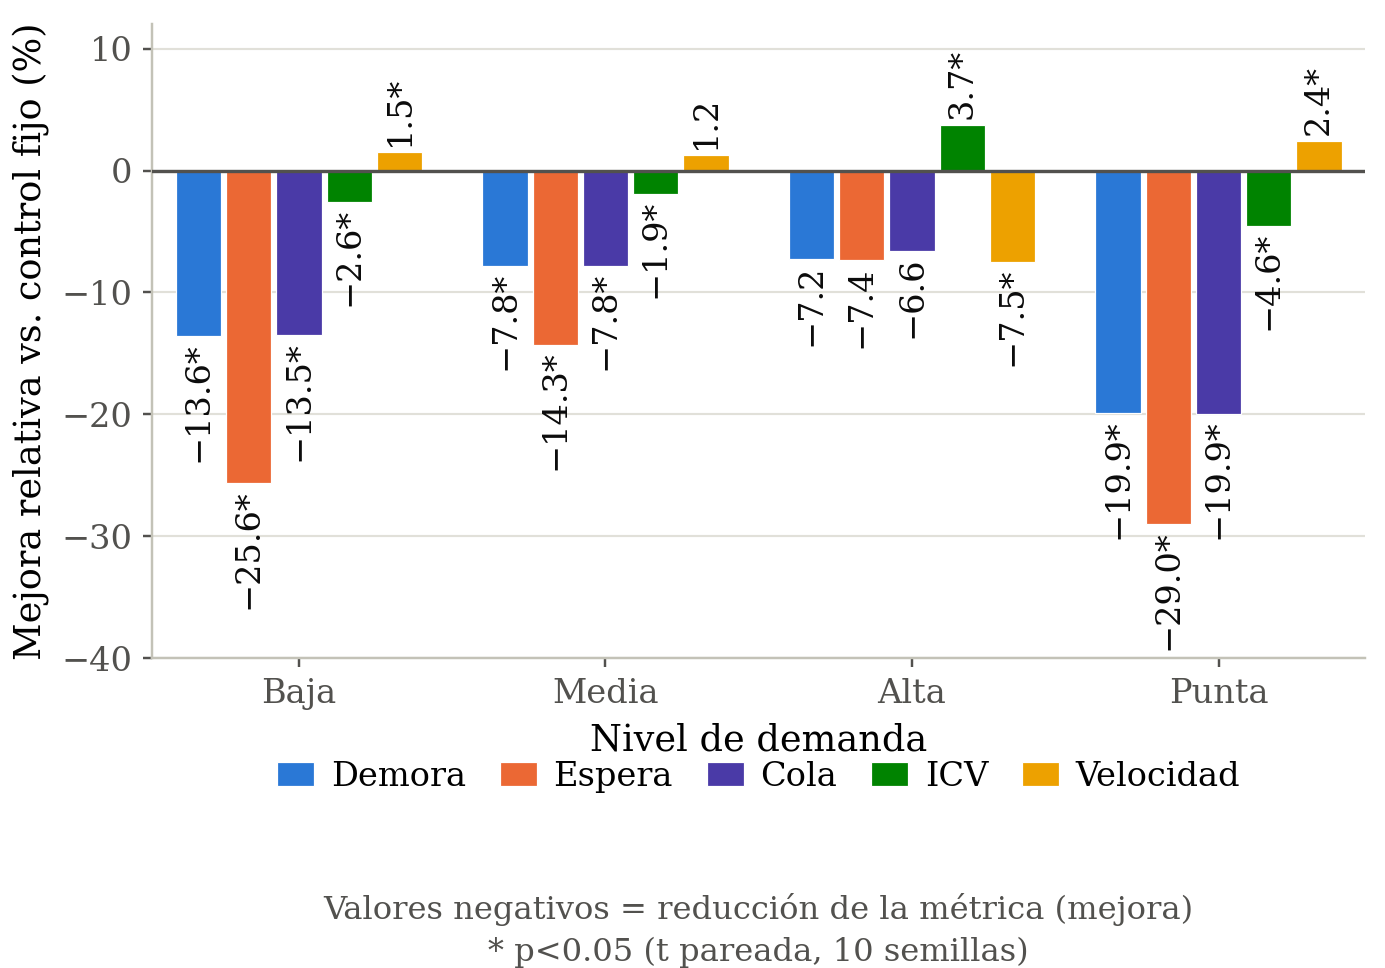
\includegraphics[width=0.92\linewidth,keepaspectratio]{media/fig_campania_demanda.png}
  \caption{Mejora del control difuso frente al plan fijo por nivel de demanda (escenario \emph{cruce-simple}, 10 semillas pareadas). El asterisco indica significancia ($p<0.05$, prueba t pareada).}
  \label{fig:campania-demanda}
\end{figure}

El patrón es nítido y honesto. El beneficio es máximo en los regímenes de flujo libre a moderado y en la
punta: la espera media cae un $25.6\%$ (baja) y un $29.0\%$ (punta), y la demora un $13.6\%$ y un $19.9\%$
respectivamente, con $p<0.001$ y mejora en las 10 réplicas. En demanda media el beneficio persiste
(espera $-14.3\%$, $p<0.001$) aunque más moderado. En cambio, bajo \emph{saturación} (demanda alta) el
comportamiento se invierte parcialmente: las reducciones de demora, espera y cola dejan de ser
significativas y, de forma notable, el ICV de red \emph{sube} un $3.7\%$ y la velocidad media \emph{cae} un
$7.5\%$ (ambos significativos), mientras que el throughput aumenta un $0.7\%$ ($p<0.05$). La lectura es
directa: con la red congestionada, la redistribución difusa prioriza vaciar la cola dominante y evacuar más
vehículos, pero lo hace a costa del acceso perpendicular, penalización que el ICV y la velocidad agregada
capturan. Este resultado, coherente con lo observado en Lima-Centro, delimita el alcance de la propuesta: el
control difuso alivia la red en los regímenes no saturados y en la punta, y debe ceder ante políticas
orientadas a throughput cuando la saturación es sostenida. En los cuatro regímenes, los límites duros de
verde $[10,120]$~s se mantuvieron sin excepción.

\subsection{Capa predictiva CNN--LSTM: evaluación y resultado}\label{subsec:ia-evaluacion}

El núcleo difuso se diseñó como un lazo reactivo: en cada intervalo de control decide a partir del estado
observado. Sobre él se implementó y entrenó una capa predictiva CNN--LSTM (descrita en el Capítulo~6) con
el fin de anticipar la congestión un horizonte corto hacia adelante y, potencialmente, preacondicionar la
decisión. Su aporte se midió por \emph{ablación pareada} en dos marcos independientes.

\textbf{Ablación en la campaña Lima-Centro.} La campaña multilínea-base ejecutó, con las mismas semillas,
el controlador propuesto con la capa predictiva activa (\texttt{difuso\_ia}) y con ella desactivada
(\texttt{difuso\_ia\_off}). El resultado es concluyente: en demanda alta ambos producen \emph{exactamente
el mismo resultado} en las 30 semillas, porque la capa predictiva permaneció operativamente inactiva ---la
compuerta por régimen de tráfico y el llenado del \emph{buffer} de secuencia (con 700 pasos e intervalo de
25~s hay solo $\sim$28 decisiones por episodio) impidieron emitir predicciones, y el controlador recurrió a
su decisión reactiva en cada caso, con traza del motivo---. En demanda media la diferencia es de $-0.81\%$
de demora y no es significativa ($p=0.48$, prueba t pareada). Por tanto, \textbf{el segundo puesto de la
campaña corresponde al núcleo difuso endurecido (selección acíclica, \emph{gap-out}, extensión por cola,
anti-inanición y transiciones seguras) y no a la capa predictiva}, y así se declara: la CNN--LSTM operó
como una guardia inactiva con degradación segura verificada.

\textbf{Ablación en la intersección aislada.} De forma complementaria, sobre \emph{cruce-simple} se comparó
el difuso con la capa predictiva activa (\emph{difuso predictivo}) contra el difuso puro, con idénticas
semillas y en los cuatro niveles de demanda. La Tabla~\ref{tab:ia-vs-difuso} resume el contraste.

\begin{table}[H]
  \centering
  \caption{Aporte de la capa predictiva CNN--LSTM sobre el control difuso (escenario \emph{cruce-simple}, 10 semillas pareadas). Variación del difuso predictivo respecto del difuso puro.}
  \label{tab:ia-vs-difuso}
  \begin{tabularx}{\linewidth}{@{}X r r r@{}}
    \toprule
    \textbf{Demanda} & \textbf{Demora} & \textbf{Espera} & \textbf{ICV}\\
    \midrule
    Baja  & $-0.4\%$ & $-0.9\%$ & $+0.4\%$\\
    Media & $-0.6\%$ & $-0.2\%$ & $-0.1\%$\\
    Alta  & $+0.5\%$ & $+0.7\%$ & $-0.4\%$\\
    Punta & $+0.1\%$ & $+0.1\%$ & $+0.0\%$\\
    \bottomrule
  \end{tabularx}
  \fuente{Elaboración propia a partir de simulación en SUMO. Ninguna diferencia es estadísticamente significativa ($p>0.05$ en las 24 comparaciones; el IC95 de la diferencia de medias cruza el cero en todas).}
\end{table}

\begin{figure}[H]
  \centering
  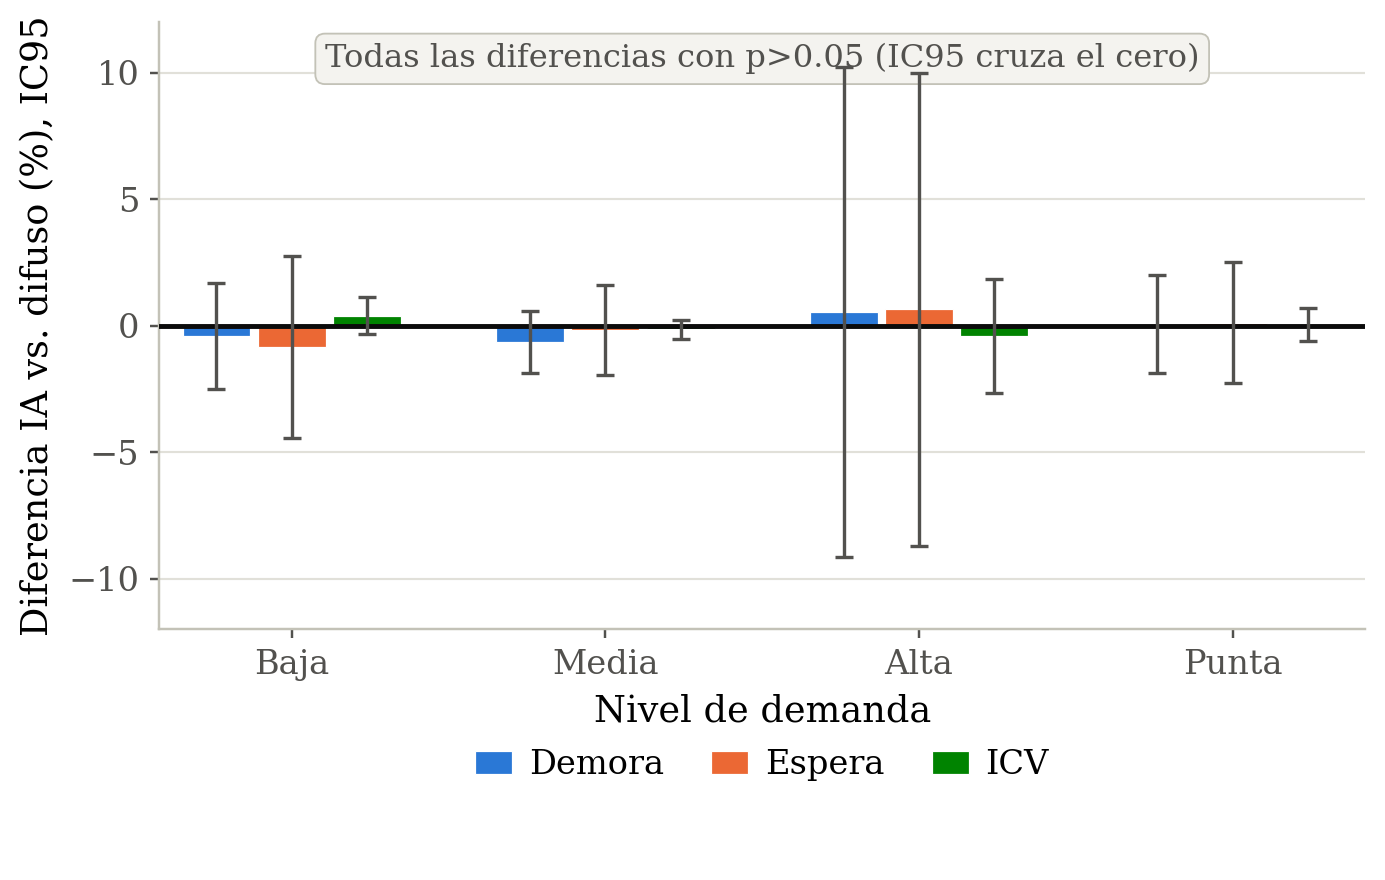
\includegraphics[width=0.90\linewidth,keepaspectratio]{media/fig_ia_nula.png}
  \caption{Diferencia del difuso predictivo (CNN--LSTM) respecto del difuso puro con su intervalo de confianza al 95\%. Todas las barras de error cruzan el cero: el aporte no es estadísticamente distinguible.}
  \label{fig:ia-nula}
\end{figure}

El resultado es un hallazgo negativo, consistente en ambos marcos, que se reporta con transparencia: la capa
predictiva \textbf{no mejora de forma medible} al control difuso reactivo. En la intersección aislada las
diferencias son del orden de las décimas de punto porcentual y ninguna alcanza significancia estadística; los
intervalos de confianza al $95\%$ contienen el cero en las veinticuatro comparaciones. La interpretación es coherente con la naturaleza
del escenario: cuando el sensado es local e inmediato y el difuso ya reacciona dentro de un intervalo de
control al estado observado, anticipar el ICV un horizonte corto no añade información accionable. El valor
esperable de la predicción aparece en un contexto distinto ---corredores coordinados, latencia de
comunicación o preacondicionamiento de olas verdes a escala de red---, que es precisamente el que se plantea
como trabajo futuro. En consecuencia, la capa CNN--LSTM se conserva como un \emph{módulo opcional} de la
arquitectura, con degradación segura verificada (su ausencia o una normalización desalineada la desactivan
sin detener el control; véase la Sección~\ref{sec:verificacion-software}), y no como un requisito del núcleo,
cuyo objetivo se cumple íntegramente con el control difuso local.

\section{Verificación del software de control}\label{sec:verificacion-software}

La comparación en SUMO evalúa el \emph{desempeño} del control; de forma complementaria, la corrección del
software se verifica con una suite de pruebas automatizadas independiente del resultado de tráfico. La suite
(ejecutada con \emph{pytest}) comprende \textbf{26 pruebas, todas satisfactorias}, y comprueba los
invariantes de seguridad funcional y la reproducibilidad del aparato experimental. La
Tabla~\ref{tab:suite-pruebas} las agrupa por familia.

\begin{table}[H]
  \centering
  \caption{Suite de verificación automatizada del núcleo de control (26 pruebas, 26 satisfactorias).}
  \label{tab:suite-pruebas}
  \begin{tabularx}{\linewidth}{@{}p{0.30\linewidth} c X@{}}
    \toprule
    \textbf{Familia} & \textbf{N.\textsuperscript{o}} & \textbf{Invariante verificado}\\
    \midrule
    Seguridad funcional & 6 & El verde se acota a $[10,120]$~s (máximo y mínimo); un valor \texttt{NaN} cae al mínimo seguro con traza; el ámbar y el todo-rojo respetan sus mínimos; se rechaza el verde simultáneo en fases incompatibles (NS/EO); y ante estado inválido o salida difusa ausente se entra en modo seguro.\\
    Transición segura & 5 & El ámbar sintético que se inserta al perder el verde nunca genera un verde nuevo; se detecta correctamente la fase de todo-rojo posterior al ámbar.\\
    Invariantes sobre SUMO real & 5 & Ejecutando el controlador sobre \emph{cruce-simple}: cero errores de paso; nunca se pasa de verde a rojo sin ámbar; el ámbar dura $\geq 3$~s; se sirve la fase de todo-rojo del programa; y el verde mínimo servido es $\geq 10$~s.\\
    Degradación de la CNN--LSTM & 5 & La ausencia del modelo no detiene el control (la IA queda inactiva); el modo \emph{off} no carga el predictor; los parámetros de seguridad se fuerzan igualmente; una normalización desalineada desactiva la IA y una correcta la activa.\\
    Métricas y reproducibilidad & 5 & El flujo por cruces queda acotado y no se satura con un solo vehículo; los eventos de validez exponen las claves correctas; una misma semilla reproduce el mismo resultado (determinismo) y semillas distintas producen resultados distintos; cada corrida registra la versión de SUMO y el \emph{hash} de \emph{git}.\\
    \bottomrule
  \end{tabularx}
  \fuente{Elaboración propia (suite \emph{pytest} del repositorio de la tesis).}
\end{table}

Estas pruebas aportan evidencia \emph{ejecutable} de la premisa de seguridad por diseño: los límites duros y
las transiciones seguras se cumplen con independencia de la recomendación difusa o de la disponibilidad de la
capa predictiva, y el aparato de medición es determinista y trazable por semilla. Con ello, los requisitos de
control y de degradación segura (R-C03, R-C04 y R-CAM04) quedan respaldados no solo por diseño, sino por una
verificación reproducible en cada ejecución.

\section{Caso de pérdida de conectividad (modo degradado)}\label{sec:modo-degradado}

El caso~D evalúa la autonomía del sistema ante la pérdida del enlace con la nube durante la
operación del control difuso. El principio de diseño es que la capa de nube solo aporta
recomendaciones de coordinación global; el control local difuso y, por encima de él, el
controlador semafórico, operan de forma autónoma. La Tabla~\ref{tab:degradacion} resume el
comportamiento esperado y verificado ante distintos modos de falla.

\begin{table}[H]
  \centering
  \caption{Comportamiento del sistema ante fallas y modo degradado.}
  \label{tab:degradacion}
  \begin{tabularx}{\linewidth}{@{}p{0.30\linewidth} X@{}}
    \toprule
    \textbf{Prueba de degradación} & \textbf{Resultado y criterio}\\
    \midrule
    Pérdida de nube durante la operación & El control continúa localmente con la última política difusa válida; ante ausencia prolongada retorna al plan base sin estados incompatibles y registra el evento. Cumple.\\
    Datos de sensado inválidos & Se inhibe la adaptación difusa y se mantiene el plan base, generando alerta de calidad de sensado. Cumple (diseño).\\
    Parámetro remoto fuera de rango & La guardia de seguridad rechaza el valor (verde acotado a [10, 120]~s) y registra el evento. Cumple (validado en SUMO).\\
    Recomendación vencida o duplicada & Se rechaza por vigencia o número de secuencia, conservando la última recomendación válida. Cumple (diseño).\\
    \bottomrule
  \end{tabularx}
  \fuente{Elaboración propia.}
\end{table}

El resultado clave es que la pérdida de conectividad no detiene el control: la autoridad de
seguridad reside en el controlador local y la simulación confirma el acotamiento de los verdes
a sus límites duros con independencia de la disponibilidad de la nube.

\section{Matriz de cumplimiento de requerimientos}\label{sec:matriz-cumplimiento}

La matriz de la Tabla~\ref{tab:cumplimiento} clasifica cada requisito en una de tres
categorías: \emph{Cumple (diseño)} cuando existe propuesta, cálculo o arquitectura
documentada; \emph{Cumple (validado en SUMO)} cuando existe una medición reproducible bajo el
protocolo del §\ref{sec:protocolo-validacion}; y \emph{Fuera de alcance (prototipo/auditoría)}
cuando el cierre requiere fabricación física o auditoría externa no ejecutada en esta tesis.

\begin{longtable}{@{}l >{\raggedright\arraybackslash}p{0.21\linewidth} l >{\raggedright\arraybackslash}p{0.47\linewidth}@{}}
  \caption{Matriz de cumplimiento de requerimientos del sistema.}
  \label{tab:cumplimiento}\\
    \toprule
    \textbf{Req.} & \textbf{Subsistema} & \textbf{Estado} & \textbf{Evidencia / observación}\\
    \midrule
  \endfirsthead
    \multicolumn{4}{@{}l}{\footnotesize\itshape (Tabla~\ref{tab:cumplimiento}, continuación)}\\
    \toprule
    \textbf{Req.} & \textbf{Subsistema} & \textbf{Estado} & \textbf{Evidencia / observación}\\
    \midrule
  \endhead
    \midrule
    \multicolumn{4}{r@{}}{\footnotesize\itshape (continúa en la página siguiente)}\\
  \endfoot
    \bottomrule
  \endlastfoot
    R-F01   & Sensado            & Validado en SUMO   & Cadena cámara$\rightarrow$ICV demostrada con video real y replicada en SUMO.\\
    R-F02   & Procesamiento local & Validado en SUMO  & Casos de ICV (8) y análisis de sensibilidad coherentes.\\
    R-F03   & Plataforma         & Cumple (diseño)    & Plataforma web con históricos y exportación CSV/JSON.\\
    R-C01   & Control            & Validado en SUMO   & Caso B y modo degradado (caso D) ejecutados.\\
    R-C02   & Arquitectura       & Cumple (diseño)    & El controlador conserva la autoridad final; integración comercial pendiente.\\
    R-C03   & Control            & Validado en SUMO   & Barrido de reglas con saturaciones; verde acotado a [10, 120]~s.\\
    R-C04   & Control            & Cumple (diseño)    & Ante sensado inválido se inhibe la adaptación y se mantiene el plan base.\\
    R-COM01 & Comunicación       & Cumple (diseño)    & Publicación de telemetría definida en la arquitectura.\\
    R-COM02 & Comunicación/seguridad & Cumple (diseño) & Rechazo de parámetros inválidos y vencidos por vigencia/secuencia.\\
    R-NUB01 & Nube               & Cumple (diseño)    & Dashboard, histórico y alertas diseñados; disponibilidad por demostrar.\\
    R-SEC01 & Ciberseguridad     & Cumple (diseño)    & Arquitectura TLS, autenticación mutua y control de acceso definida.\\
    R-SEC05 & Ciberseguridad     & Fuera de alcance   & Auditoría, \textit{pentesting} y conformidad IEC 62443 no ejecutados (piloto).\\
    R-SEC02 & Ciberseguridad     & Cumple (diseño)    & Modelo de amenazas documentado.\\
    R-SEC03 & Ciberseguridad     & Cumple (diseño)    & Registro de eventos y trazabilidad definidos.\\
    R-SEC04 & Ciberseguridad     & Cumple (diseño)    & Separación de roles y autoridad documentada.\\
    R-ELEC01 & Energía           & Cumple (diseño)    & Esquema eléctrico y coordinación de protecciones.\\
    R-ELEC02 & Energía           & Cumple (diseño)    & Balance de potencia y autonomía por UPS calculados.\\
    R-ELEC03 & Electrónica       & Cumple (diseño)    & PCB, distribución y diagnóstico definidos.\\
    R-MEC01 & Mecánico           & Cumple (diseño)    & CAD y acceso de mantenimiento resueltos.\\
    R-MEC02 & Mecánico           & Fuera de alcance   & Certificación IP65/IK10 y resistencia al vandalismo no ensayadas; requieren prototipo.\\
    R-MEC03 & Mecánico/sensado   & Cumple (diseño)    & Cobertura, torque y resistencia dimensionados.\\
    R-CAM01 & Mecánico/Control   & Cumple (diseño)    & Sistema de orientación (NEMA~23, biela-manivela, rodamiento) dimensionado en el Cap.~5.\\
    R-CAM02 & Percepción         & Cumple (diseño)    & Política de estados \textit{MOVING}/\textit{SETTLING}/\textit{OBSERVING} definida en el Cap.~6.\\
    R-CAM03 & Control            & Cumple (diseño)    & Vigencia temporal $T_{valid}$ por vector de estado de eje.\\
    R-CAM04 & Seg.\ funcional    & Cumple (diseño)    & Degradación por baja confianza ($\tau_{det}$) definida en el Cap.~6.\\
    R-OP01  & Operación          & Cumple (diseño)    & Procedimiento de mantenimiento preventivo definido.\\
    R-VAL01 & Validación         & Validado en SUMO   & Casos A y B reproducibles (Tabla~\ref{tab:resultados-ab}).\\
    R-VAL02 & Validación         & Validado en SUMO   & Resultados comparativos consolidados.\\
    R-VAL03 & Validación         & Cumple (diseño)    & Modo degradado (caso D) verificado a nivel de comportamiento.\\
    R-COST01 & Costos            & Cumple (diseño)    & CAPEX/OPEX consolidados en el §\ref{cap:analisis-economico}.\\
\end{longtable}
\fuente{Elaboración propia.}

\section{Análisis de costos}\label{cap:analisis-economico}

El análisis económico contempla la inversión inicial por intersección (CAPEX), los costos
operativos recurrentes (OPEX) y la infraestructura de nube compartida. Para evitar ambigüedad,
el costo del primer año se reporta en dos niveles: \textbf{sin la fracción prorrateada de nube},
cada intersección demanda \textbf{aproximadamente S/ 16\,500} (S/ 14\,594 de CAPEX más S/ 1\,940
de OPEX local), que se redondea a la cifra de referencia de \textbf{S/ 17\,000}; \textbf{con la
fracción de nube} (S/ 3\,178 anuales por intersección), el primer año asciende a
\textbf{unos S/ 19\,700}. La nube se contabiliza de forma explícita y separada por ser un recurso
centralizado que se prorratea entre toda la red.

Esta cifra representa una optimización significativa respecto de los sistemas adaptativos
tradicionales, que típicamente superan los S/ 30\,000 por intersección. El ahorro proviene de
tres decisiones de diseño: aprovechar el controlador semafórico certificado existente (el
módulo solo sensa, procesa y recomienda), simplificar la estructura mecánica con fabricación
local y reducir la cimentación gracias al menor peso del conjunto. En la distribución del
CAPEX, la estructura mecánica concentra el 33.2\%, seguida por la instalación (23.5\%) y el
sistema de visión (21.7\%), proporción característica de un equipo que prioriza robustez física
ante la contaminación, las vibraciones y el clima del entorno urbano limeño.

\subsection{Costos de capital (CAPEX)}

La Tabla~\ref{tab:capex} resume el CAPEX agrupado en siete rubros de \emph{nivel de proyecto}, que
incorporan además la estructura, la obra de instalación y la integración; por ello sus cifras no
coinciden ítem a ítem con la estimación de componentes electrónicos del Capítulo~4
(Tabla~\ref{tab:costos-electronica}, $\approx$~S/~6\,565), que constituye un subtotal de referencia
distribuido entre los rubros de sistema de visión, electrónica de control, protección eléctrica y
sensores. El respaldo energético (UPS APC SMT1500IC, S/~2\,279.99) es el ítem electrónico de mayor costo y se
contabiliza una sola vez dentro de dicho subtotal; los rubros de la Tabla~\ref{tab:capex} son una estimación de
nivel de proyecto y no la suma directa de los componentes del Capítulo~4. El desglose
fino, con los más de cuarenta ítems individuales (gabinete, postes, cámara, motorización, SBC, módulo
4G, protecciones, sensores y partidas de obra), se traslada al Anexo~D (Presupuesto detallado) para no
recargar la lectura.

\begin{table}[H]
  \centering
  \caption{CAPEX por intersección, agrupado por rubro.}
  \label{tab:capex}
  \begin{tabularx}{\linewidth}{@{}X r r@{}}
    \toprule
    \textbf{Rubro} & \textbf{Costo (S/)} & \textbf{\% del total}\\
    \midrule
    Estructura mecánica (gabinete, poste, giro, anclajes) & 4\,850 & 33.2\%\\
    Instalación y puesta en marcha (obra civil, montaje, calibración) & 3\,436 & 23.5\%\\
    Sistema de visión (cámara, motorización y óptica) & 3\,165 & 21.7\%\\
    Electrónica de control (SBC, módulo 4G, PCB, alimentación y respaldo) & 2\,172 & 14.9\%\\
    Protección eléctrica (breaker, diferencial, DPS, borneras) & 630 & 4.3\%\\
    Sensores e instrumentación (corriente, ultrasónico, temperatura, ventilación) & 341 & 2.3\%\\
    \midrule
    \textbf{Total CAPEX por intersección} & \textbf{14\,594} & \textbf{100.0\%}\\
    \bottomrule
  \end{tabularx}
  \fuente{Elaboración propia.}
\end{table}

A la inversión por intersección se añade la infraestructura de nube, que constituye el cerebro
centralizado del sistema y procesa la telemetría de la red completa (del orden de 50
intersecciones). Esta capa es un costo compartido, no un CAPEX por intersección: su detalle por
servicio (IoT Hub, Stream Analytics, bases de datos, almacenamiento, cómputo de \emph{machine
learning} y observabilidad) asciende a unos S/ 13\,243 mensuales (S/ 158\,916 anuales) para toda
la red y se documenta en el Anexo~D. Prorrateada entre las intersecciones equivale a unos
S/ 265 mensuales por intersección, monto que se incorpora como rubro de nube dentro del OPEX.

\subsection{Costos operativos anuales (OPEX)}

Los costos operativos garantizan la disponibilidad del sistema durante todo el año. La
Tabla~\ref{tab:opex} consolida los cuatro componentes recurrentes por intersección, incluida
la fracción prorrateada de nube.

\begin{table}[H]
  \centering
  \caption{OPEX anual por intersección, con subtotal local y total con nube prorrateada.}
  \label{tab:opex}
  \begin{tabularx}{\linewidth}{@{}X X r@{}}
    \toprule
    \textbf{Categoría} & \textbf{Concepto} & \textbf{Costo anual (S/)}\\
    \midrule
    Energía eléctrica & 150~W $\times$ 24~h $\times$ 365~d @ S/ 0.70/kWh (tarifa BT5B) & 920\\
    Conectividad 4G & Plan de datos 10~GB/mes @ S/ 45/mes & 540\\
    Mantenimiento & Inspección trimestral preventiva y limpieza de ópticas & 480\\
    \midrule
    \textbf{Subtotal OPEX local (sin nube)} & & \textbf{1\,940}\\
    Nube (prorrateada) & Fracción por intersección de la infraestructura compartida & 3\,178\\
    \midrule
    \textbf{Total OPEX anual (con nube)} & & \textbf{5\,118}\\
    \bottomrule
  \end{tabularx}
  \fuente{Elaboración propia.}
\end{table}

La energía eléctrica es el mayor componente del OPEX local (47.4\%): el consumo de 150~W
integra la SBC (25~W), la cámara con iluminación infrarroja (40~W), la motorización en
\emph{standby} (5~W), el módulo 4G (8~W) y las pérdidas del UPS (15~W), con margen de
seguridad. La conectividad 4G (27.8\%) y el mantenimiento preventivo (24.7\%) completan el
gasto local. De este modo, el primer año \emph{sin} nube suma CAPEX (S/ 14\,594) más OPEX local
(S/ 1\,940) $\approx$ S/ 16\,500, redondeado a la cifra de referencia de S/ 17\,000; incorporando
la fracción prorrateada de nube (S/ 3\,178), el primer año \emph{con} nube asciende a unos
S/ 19\,700 por intersección. Los años siguientes, ya sin CAPEX, cuestan el OPEX anual: S/ 1\,940
locales o S/ 5\,118 con nube.

Quedan fuera del costeo explícito algunas partidas indirectas relevantes para un despliegue
real: la coordinación interinstitucional (Municipalidad, Policía, SUTRAN), la eventual
adecuación de la infraestructura eléctrica en ciertas intersecciones y la capacitación
continua de operadores para interpretar métricas, usar los \emph{dashboards} y responder a las
alertas.
